\documentclass[1p]{elsarticle_modified}
%\bibliographystyle{elsarticle-num}

%\usepackage[colorlinks]{hyperref}
%\usepackage{abbrmath_seonhwa} %\Abb, \Ascr, \Acal ,\Abf, \Afrak
\usepackage{amsfonts}
\usepackage{amssymb}
\usepackage{amsmath}
\usepackage{amsthm}
\usepackage{scalefnt}
\usepackage{amsbsy}
\usepackage{kotex}
\usepackage{caption}
\usepackage{subfig}
\usepackage{color}
\usepackage{graphicx}
\usepackage{xcolor} %% white, black, red, green, blue, cyan, magenta, yellow
\usepackage{float}
\usepackage{setspace}
\usepackage{hyperref}

\usepackage{tikz}
\usetikzlibrary{arrows}

\usepackage{multirow}
\usepackage{array} % fixed length table
\usepackage{hhline}

%%%%%%%%%%%%%%%%%%%%%
\makeatletter
\renewcommand*\env@matrix[1][\arraystretch]{%
	\edef\arraystretch{#1}%
	\hskip -\arraycolsep
	\let\@ifnextchar\new@ifnextchar
	\array{*\c@MaxMatrixCols c}}
\makeatother %https://tex.stackexchange.com/questions/14071/how-can-i-increase-the-line-spacing-in-a-matrix
%%%%%%%%%%%%%%%

\usepackage[normalem]{ulem}

\newcommand{\msout}[1]{\ifmmode\text{\sout{\ensuremath{#1}}}\else\sout{#1}\fi}
%SOURCE: \msout is \stkout macro in https://tex.stackexchange.com/questions/20609/strikeout-in-math-mode

\newcommand{\cancel}[1]{
	\ifmmode
	{\color{red}\msout{#1}}
	\else
	{\color{red}\sout{#1}}
	\fi
}

\newcommand{\add}[1]{
	{\color{blue}\uwave{#1}}
}

\newcommand{\replace}[2]{
	\ifmmode
	{\color{red}\msout{#1}}{\color{blue}\uwave{#2}}
	\else
	{\color{red}\sout{#1}}{\color{blue}\uwave{#2}}
	\fi
}

\newcommand{\Sol}{\mathcal{S}} %segment
\newcommand{\D}{D} %diagram
\newcommand{\A}{\mathcal{A}} %arc


%%%%%%%%%%%%%%%%%%%%%%%%%%%%%5 test

\def\sl{\operatorname{\textup{SL}}(2,\Cbb)}
\def\psl{\operatorname{\textup{PSL}}(2,\Cbb)}
\def\quan{\mkern 1mu \triangleright \mkern 1mu}

\theoremstyle{definition}
\newtheorem{thm}{Theorem}[section]
\newtheorem{prop}[thm]{Proposition}
\newtheorem{lem}[thm]{Lemma}
\newtheorem{ques}[thm]{Question}
\newtheorem{cor}[thm]{Corollary}
\newtheorem{defn}[thm]{Definition}
\newtheorem{exam}[thm]{Example}
\newtheorem{rmk}[thm]{Remark}
\newtheorem{alg}[thm]{Algorithm}

\newcommand{\I}{\sqrt{-1}}
\begin{document}

%\begin{frontmatter}
%
%\title{Boundary parabolic representations of knots up to 8 crossings}
%
%%% Group authors per affiliation:
%\author{Yunhi Cho} 
%\address{Department of Mathematics, University of Seoul, Seoul, Korea}
%\ead{yhcho@uos.ac.kr}
%
%
%\author{Seonhwa Kim} %\fnref{s_kim}}
%\address{Center for Geometry and Physics, Institute for Basic Science, Pohang, 37673, Korea}
%\ead{ryeona17@ibs.re.kr}
%
%\author{Hyuk Kim}
%\address{Department of Mathematical Sciences, Seoul National University, Seoul 08826, Korea}
%\ead{hyukkim@snu.ac.kr}
%
%\author{Seokbeom Yoon}
%\address{Department of Mathematical Sciences, Seoul National University, Seoul, 08826,  Korea}
%\ead{sbyoon15@snu.ac.kr}
%
%\begin{abstract}
%We find all boundary parabolic representation of knots up to 8 crossings.
%
%\end{abstract}
%\begin{keyword}
%    \MSC[2010] 57M25 
%\end{keyword}
%
%\end{frontmatter}

%\linenumbers
%\tableofcontents
%
\newcommand\colored[1]{\textcolor{white}{\rule[-0.35ex]{0.8em}{1.4ex}}\kern-0.8em\color{red} #1}%
%\newcommand\colored[1]{\textcolor{white}{ #1}\kern-2.17ex	\textcolor{white}{ #1}\kern-1.81ex	\textcolor{white}{ #1}\kern-2.15ex\color{red}#1	}

{\Large $\underline{12a_{1130}~(K12a_{1130})}$}

\setlength{\tabcolsep}{10pt}
\renewcommand{\arraystretch}{1.6}
\vspace{1cm}\begin{tabular}{m{100pt}>{\centering\arraybackslash}m{274pt}}
\multirow{5}{120pt}{
	\centering
	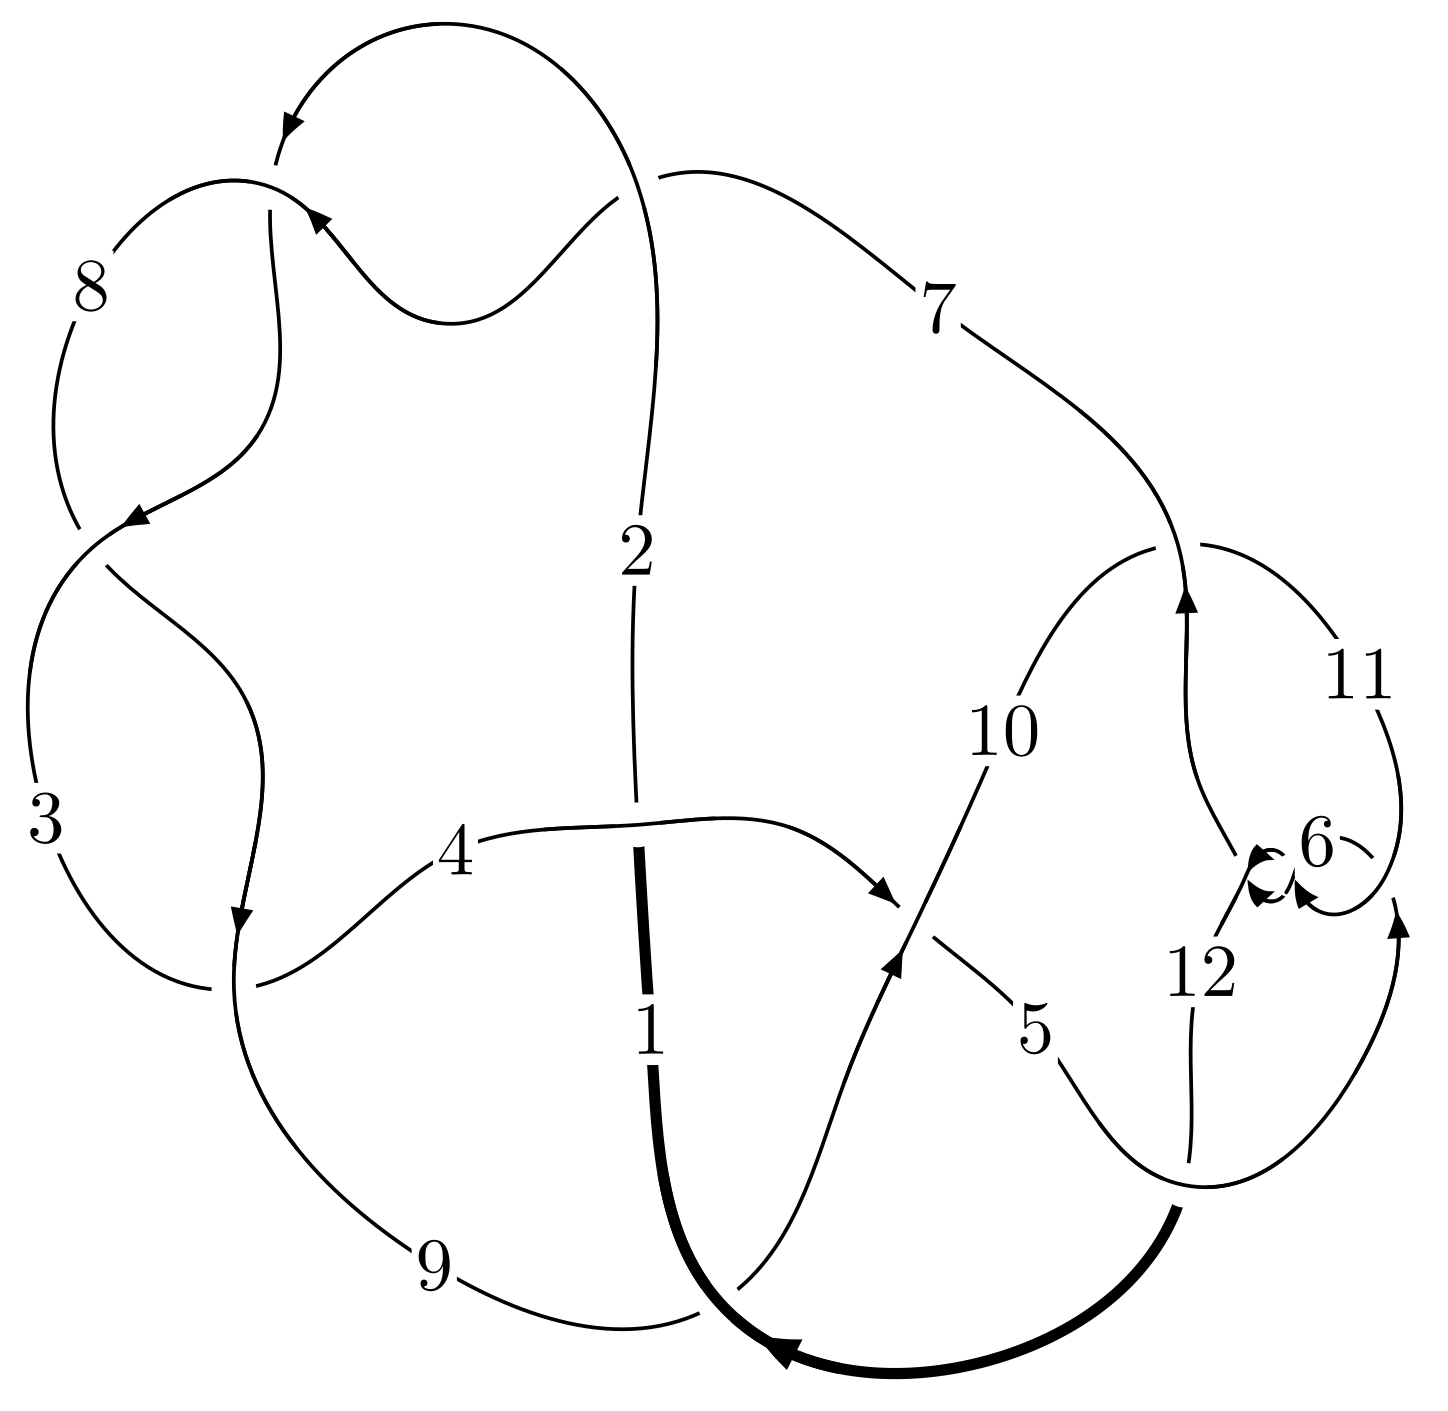
\includegraphics[width=112pt]{../../../GIT/diagram.site/Diagrams/png/1931_12a_1130.png}\\
\ \ \ A knot diagram\footnotemark}&
\allowdisplaybreaks
\textbf{Linearized knot diagam} \\
\cline{2-2}
 &
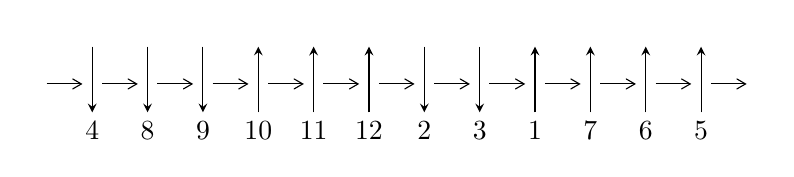
\begin{tikzpicture}[x=20pt, y=17pt]
	% nodes
	\node (C0) at (0, 0) {};
	\node (C1) at (1, 0) {};
	\node (C1U) at (1, +1) {};
	\node (C1D) at (1, -1) {4};

	\node (C2) at (2, 0) {};
	\node (C2U) at (2, +1) {};
	\node (C2D) at (2, -1) {8};

	\node (C3) at (3, 0) {};
	\node (C3U) at (3, +1) {};
	\node (C3D) at (3, -1) {9};

	\node (C4) at (4, 0) {};
	\node (C4U) at (4, +1) {};
	\node (C4D) at (4, -1) {10};

	\node (C5) at (5, 0) {};
	\node (C5U) at (5, +1) {};
	\node (C5D) at (5, -1) {11};

	\node (C6) at (6, 0) {};
	\node (C6U) at (6, +1) {};
	\node (C6D) at (6, -1) {12};

	\node (C7) at (7, 0) {};
	\node (C7U) at (7, +1) {};
	\node (C7D) at (7, -1) {2};

	\node (C8) at (8, 0) {};
	\node (C8U) at (8, +1) {};
	\node (C8D) at (8, -1) {3};

	\node (C9) at (9, 0) {};
	\node (C9U) at (9, +1) {};
	\node (C9D) at (9, -1) {1};

	\node (C10) at (10, 0) {};
	\node (C10U) at (10, +1) {};
	\node (C10D) at (10, -1) {7};

	\node (C11) at (11, 0) {};
	\node (C11U) at (11, +1) {};
	\node (C11D) at (11, -1) {6};

	\node (C12) at (12, 0) {};
	\node (C12U) at (12, +1) {};
	\node (C12D) at (12, -1) {5};
	\node (C13) at (13, 0) {};

	% arrows
	\draw[->,>={angle 60}]
	(C0) edge (C1) (C1) edge (C2) (C2) edge (C3) (C3) edge (C4) (C4) edge (C5) (C5) edge (C6) (C6) edge (C7) (C7) edge (C8) (C8) edge (C9) (C9) edge (C10) (C10) edge (C11) (C11) edge (C12) (C12) edge (C13) ;	\draw[->,>=stealth]
	(C1U) edge (C1D) (C2U) edge (C2D) (C3U) edge (C3D) (C4D) edge (C4U) (C5D) edge (C5U) (C6D) edge (C6U) (C7U) edge (C7D) (C8U) edge (C8D) (C9D) edge (C9U) (C10D) edge (C10U) (C11D) edge (C11U) (C12D) edge (C12U) ;
	\end{tikzpicture} \\
\hhline{~~} \\& 
\textbf{Solving Sequence} \\ \cline{2-2} 
 &
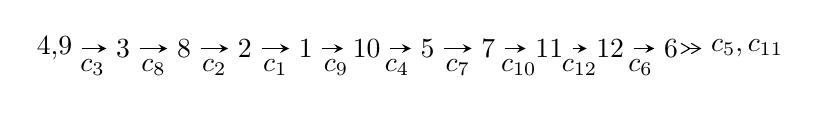
\begin{tikzpicture}[x=22pt, y=7pt]
	% node
	\node (A0) at (-1/8, 0) {4,9};
	\node (A1) at (1, 0) {3};
	\node (A2) at (2, 0) {8};
	\node (A3) at (3, 0) {2};
	\node (A4) at (4, 0) {1};
	\node (A5) at (5, 0) {10};
	\node (A6) at (6, 0) {5};
	\node (A7) at (7, 0) {7};
	\node (A8) at (8, 0) {11};
	\node (A9) at (9, 0) {12};
	\node (A10) at (10, 0) {6};
	\node (C1) at (1/2, -1) {$c_{3}$};
	\node (C2) at (3/2, -1) {$c_{8}$};
	\node (C3) at (5/2, -1) {$c_{2}$};
	\node (C4) at (7/2, -1) {$c_{1}$};
	\node (C5) at (9/2, -1) {$c_{9}$};
	\node (C6) at (11/2, -1) {$c_{4}$};
	\node (C7) at (13/2, -1) {$c_{7}$};
	\node (C8) at (15/2, -1) {$c_{10}$};
	\node (C9) at (17/2, -1) {$c_{12}$};
	\node (C10) at (19/2, -1) {$c_{6}$};
	\node (A11) at (45/4, 0) {$c_{5},c_{11}$};

	% edge
	\draw[->,>=stealth]	
	(A0) edge (A1) (A1) edge (A2) (A2) edge (A3) (A3) edge (A4) (A4) edge (A5) (A5) edge (A6) (A6) edge (A7) (A7) edge (A8) (A8) edge (A9) (A9) edge (A10) ;
	\draw[->>,>={angle 60}]	
	(A10) edge (A11);
\end{tikzpicture} \\ 

\end{tabular} \\

\footnotetext{
The image of knot diagram is generated by the software ``\textbf{Draw programme}" developed by Andrew Bartholomew(\url{http://www.layer8.co.uk/maths/draw/index.htm\#Running-draw}), where we modified some parts for our purpose(\url{https://github.com/CATsTAILs/LinksPainter}).
}\phantom \\ \newline 
\centering \textbf{Ideals for irreducible components\footnotemark of $X_{\text{par}}$} 
 
\begin{align*}
I^u_{1}&=\langle 
u^{62}- u^{61}+\cdots+u+1\rangle \\
\\
\end{align*}
\raggedright * 1 irreducible components of $\dim_{\mathbb{C}}=0$, with total 62 representations.\\
\footnotetext{All coefficients of polynomials are rational numbers. But the coefficients are sometimes approximated in decimal forms when there is not enough margin.}
\newpage
\renewcommand{\arraystretch}{1}
\centering \section*{I. $I^u_{1}= \langle u^{62}- u^{61}+\cdots+u+1 \rangle$}
\flushleft \textbf{(i) Arc colorings}\\
\begin{tabular}{m{7pt} m{180pt} m{7pt} m{180pt} }
\flushright $a_{4}=$&$\begin{pmatrix}1\\0\end{pmatrix}$ \\
\flushright $a_{9}=$&$\begin{pmatrix}0\\u\end{pmatrix}$ \\
\flushright $a_{3}=$&$\begin{pmatrix}1\\- u^2\end{pmatrix}$ \\
\flushright $a_{8}=$&$\begin{pmatrix}u\\- u^3+u\end{pmatrix}$ \\
\flushright $a_{2}=$&$\begin{pmatrix}- u^2+1\\u^4-2 u^2\end{pmatrix}$ \\
\flushright $a_{1}=$&$\begin{pmatrix}u^4-3 u^2+1\\u^4-2 u^2\end{pmatrix}$ \\
\flushright $a_{10}=$&$\begin{pmatrix}u^9-6 u^7+11 u^5-6 u^3+u\\u^9-5 u^7+7 u^5-2 u^3+u\end{pmatrix}$ \\
\flushright $a_{5}=$&$\begin{pmatrix}- u^{18}+11 u^{16}-48 u^{14}+105 u^{12}-121 u^{10}+75 u^8-30 u^6+8 u^4- u^2+1\\- u^{18}+10 u^{16}-39 u^{14}+74 u^{12}-71 u^{10}+38 u^8-18 u^6+4 u^4- u^2\end{pmatrix}$ \\
\flushright $a_{7}=$&$\begin{pmatrix}- u^3+2 u\\u^5-3 u^3+u\end{pmatrix}$ \\
\flushright $a_{11}=$&$\begin{pmatrix}u^{17}-10 u^{15}+39 u^{13}-74 u^{11}+71 u^9-38 u^7+18 u^5-4 u^3+u\\- u^{19}+11 u^{17}-48 u^{15}+105 u^{13}-121 u^{11}+75 u^9-30 u^7+8 u^5- u^3+u\end{pmatrix}$ \\
\flushright $a_{12}=$&$\begin{pmatrix}u^{32}-19 u^{30}+\cdots-2 u^2+1\\u^{32}-18 u^{30}+\cdots+12 u^8-2 u^2\end{pmatrix}$ \\
\flushright $a_{6}=$&$\begin{pmatrix}- u^{54}+31 u^{52}+\cdots-2 u^2+1\\u^{56}-32 u^{54}+\cdots+6 u^4-2 u^2\end{pmatrix}$\\&\end{tabular}
\flushleft \textbf{(ii) Obstruction class $= -1$}\\~\\
\flushleft \textbf{(iii) Cusp Shapes $= -4 u^{59}+136 u^{57}+\cdots-4 u+6$}\\~\\
\newpage\renewcommand{\arraystretch}{1}
\flushleft \textbf{(iv) u-Polynomials at the component}\newline \\
\begin{tabular}{m{50pt}|m{274pt}}
Crossings & \hspace{64pt}u-Polynomials at each crossing \\
\hline $$\begin{aligned}c_{1}\end{aligned}$$&$\begin{aligned}
&u^{62}-17 u^{61}+\cdots+1847 u-113
\end{aligned}$\\
\hline $$\begin{aligned}c_{2},c_{3},c_{7}\\c_{8}\end{aligned}$$&$\begin{aligned}
&u^{62}+u^{61}+\cdots- u+1
\end{aligned}$\\
\hline $$\begin{aligned}c_{4}\end{aligned}$$&$\begin{aligned}
&u^{62}- u^{61}+\cdots+15 u+1
\end{aligned}$\\
\hline $$\begin{aligned}c_{5},c_{6},c_{11}\end{aligned}$$&$\begin{aligned}
&u^{62}+u^{61}+\cdots- u+1
\end{aligned}$\\
\hline $$\begin{aligned}c_{9}\end{aligned}$$&$\begin{aligned}
&u^{62}-5 u^{61}+\cdots+640 u+304
\end{aligned}$\\
\hline $$\begin{aligned}c_{10},c_{12}\end{aligned}$$&$\begin{aligned}
&u^{62}-3 u^{61}+\cdots+55 u-9
\end{aligned}$\\
\hline
\end{tabular}\\~\\
\newpage\renewcommand{\arraystretch}{1}
\flushleft \textbf{(v) Riley Polynomials at the component}\newline \\
\begin{tabular}{m{50pt}|m{274pt}}
Crossings & \hspace{64pt}Riley Polynomials at each crossing \\
\hline $$\begin{aligned}c_{1}\end{aligned}$$&$\begin{aligned}
&y^{62}-11 y^{61}+\cdots-256449 y+12769
\end{aligned}$\\
\hline $$\begin{aligned}c_{2},c_{3},c_{7}\\c_{8}\end{aligned}$$&$\begin{aligned}
&y^{62}-71 y^{61}+\cdots- y+1
\end{aligned}$\\
\hline $$\begin{aligned}c_{4}\end{aligned}$$&$\begin{aligned}
&y^{62}+y^{61}+\cdots+127 y+1
\end{aligned}$\\
\hline $$\begin{aligned}c_{5},c_{6},c_{11}\end{aligned}$$&$\begin{aligned}
&y^{62}-51 y^{61}+\cdots- y+1
\end{aligned}$\\
\hline $$\begin{aligned}c_{9}\end{aligned}$$&$\begin{aligned}
&y^{62}+25 y^{61}+\cdots-2665888 y+92416
\end{aligned}$\\
\hline $$\begin{aligned}c_{10},c_{12}\end{aligned}$$&$\begin{aligned}
&y^{62}+41 y^{61}+\cdots-2233 y+81
\end{aligned}$\\
\hline
\end{tabular}\\~\\
\newpage\flushleft \textbf{(vi) Complex Volumes and Cusp Shapes}
$$\begin{array}{c|c|c}  
\text{Solutions to }I^u_{1}& \I (\text{vol} + \sqrt{-1}CS) & \text{Cusp shape}\\
 \hline 
\begin{aligned}
u &= -0.708768 + 0.494433 I\end{aligned}
 & -0.01088 + 11.34630 I & \phantom{-}1.00889 - 9.72117 I \\ \hline\begin{aligned}
u &= -0.708768 - 0.494433 I\end{aligned}
 & -0.01088 - 11.34630 I & \phantom{-}1.00889 + 9.72117 I \\ \hline\begin{aligned}
u &= \phantom{-}0.712691 + 0.482290 I\end{aligned}
 & -4.59207 - 7.20372 I & -3.76784 + 7.81893 I \\ \hline\begin{aligned}
u &= \phantom{-}0.712691 - 0.482290 I\end{aligned}
 & -4.59207 + 7.20372 I & -3.76784 - 7.81893 I \\ \hline\begin{aligned}
u &= \phantom{-}0.821977 + 0.248060 I\end{aligned}
 & -1.60870 + 5.02300 I & -2.11818 - 2.33854 I \\ \hline\begin{aligned}
u &= \phantom{-}0.821977 - 0.248060 I\end{aligned}
 & -1.60870 - 5.02300 I & -2.11818 + 2.33854 I \\ \hline\begin{aligned}
u &= -0.717017 + 0.462468 I\end{aligned}
 & -1.49252 + 3.04670 I & -0.95105 - 4.03685 I \\ \hline\begin{aligned}
u &= -0.717017 - 0.462468 I\end{aligned}
 & -1.49252 - 3.04670 I & -0.95105 + 4.03685 I \\ \hline\begin{aligned}
u &= -0.804271 + 0.274945 I\end{aligned}
 & -5.95144 - 0.93191 I & -6.82947 - 0.41510 I \\ \hline\begin{aligned}
u &= -0.804271 - 0.274945 I\end{aligned}
 & -5.95144 + 0.93191 I & -6.82947 + 0.41510 I \\ \hline\begin{aligned}
u &= \phantom{-}0.786850 + 0.308644 I\end{aligned}
 & -2.51765 - 3.16231 I & -3.19226 + 4.63064 I \\ \hline\begin{aligned}
u &= \phantom{-}0.786850 - 0.308644 I\end{aligned}
 & -2.51765 + 3.16231 I & -3.19226 - 4.63064 I \\ \hline\begin{aligned}
u &= \phantom{-}0.645614 + 0.481542 I\end{aligned}
 & \phantom{-}5.40192 - 4.93284 I & \phantom{-}5.98347 + 6.95967 I \\ \hline\begin{aligned}
u &= \phantom{-}0.645614 - 0.481542 I\end{aligned}
 & \phantom{-}5.40192 + 4.93284 I & \phantom{-}5.98347 - 6.95967 I \\ \hline\begin{aligned}
u &= -0.661871 + 0.431665 I\end{aligned}
 & -0.37286 + 3.82050 I & \phantom{-}0.80971 - 8.83279 I \\ \hline\begin{aligned}
u &= -0.661871 - 0.431665 I\end{aligned}
 & -0.37286 - 3.82050 I & \phantom{-}0.80971 + 8.83279 I \\ \hline\begin{aligned}
u &= \phantom{-}0.620723 + 0.337292 I\end{aligned}
 & -1.08571 - 1.06603 I & -2.60164 + 1.01884 I \\ \hline\begin{aligned}
u &= \phantom{-}0.620723 - 0.337292 I\end{aligned}
 & -1.08571 + 1.06603 I & -2.60164 - 1.01884 I \\ \hline\begin{aligned}
u &= -0.698913\phantom{ +0.000000I}\end{aligned}
 & \phantom{-}2.99735\phantom{ +0.000000I} & \phantom{-}1.03130\phantom{ +0.000000I} \\ \hline\begin{aligned}
u &= -0.524035 + 0.459452 I\end{aligned}
 & \phantom{-}3.21307 - 1.54671 I & \phantom{-}5.20781 - 1.38178 I \\ \hline\begin{aligned}
u &= -0.524035 - 0.459452 I\end{aligned}
 & \phantom{-}3.21307 + 1.54671 I & \phantom{-}5.20781 + 1.38178 I \\ \hline\begin{aligned}
u &= -0.383395 + 0.494306 I\end{aligned}
 & \phantom{-}3.62071 + 4.90483 I & \phantom{-}6.55837 - 6.65558 I \\ \hline\begin{aligned}
u &= -0.383395 - 0.494306 I\end{aligned}
 & \phantom{-}3.62071 - 4.90483 I & \phantom{-}6.55837 + 6.65558 I \\ \hline\begin{aligned}
u &= -0.164450 + 0.582453 I\end{aligned}
 & \phantom{-}1.57732 - 7.67033 I & \phantom{-}4.62669 + 4.82288 I \\ \hline\begin{aligned}
u &= -0.164450 - 0.582453 I\end{aligned}
 & \phantom{-}1.57732 + 7.67033 I & \phantom{-}4.62669 - 4.82288 I \\ \hline\begin{aligned}
u &= \phantom{-}0.412131 + 0.432363 I\end{aligned}
 & -0.75273 - 1.50608 I & \phantom{-}0.71484 + 5.28376 I \\ \hline\begin{aligned}
u &= \phantom{-}0.412131 - 0.432363 I\end{aligned}
 & -0.75273 + 1.50608 I & \phantom{-}0.71484 - 5.28376 I \\ \hline\begin{aligned}
u &= \phantom{-}0.147128 + 0.569414 I\end{aligned}
 & -2.94806 + 3.60850 I & -0.16305 - 2.91417 I \\ \hline\begin{aligned}
u &= \phantom{-}0.147128 - 0.569414 I\end{aligned}
 & -2.94806 - 3.60850 I & -0.16305 + 2.91417 I \\ \hline\begin{aligned}
u &= \phantom{-}0.250782 + 0.527668 I\end{aligned}
 & \phantom{-}6.54621 + 1.43098 I & \phantom{-}9.71321 - 0.47730 I\\
 \hline 
 \end{array}$$\newpage$$\begin{array}{c|c|c}  
\text{Solutions to }I^u_{1}& \I (\text{vol} + \sqrt{-1}CS) & \text{Cusp shape}\\
 \hline 
\begin{aligned}
u &= \phantom{-}0.250782 - 0.527668 I\end{aligned}
 & \phantom{-}6.54621 - 1.43098 I & \phantom{-}9.71321 + 0.47730 I \\ \hline\begin{aligned}
u &= -0.116312 + 0.549646 I\end{aligned}
 & \phantom{-}0.240300 + 0.413797 I & \phantom{-}2.99515 - 0.89523 I \\ \hline\begin{aligned}
u &= -0.116312 - 0.549646 I\end{aligned}
 & \phantom{-}0.240300 - 0.413797 I & \phantom{-}2.99515 + 0.89523 I \\ \hline\begin{aligned}
u &= -1.45204\phantom{ +0.000000I}\end{aligned}
 & \phantom{-}1.51065\phantom{ +0.000000I} & \phantom{-0.000000 } 0 \\ \hline\begin{aligned}
u &= \phantom{-}1.47356 + 0.06742 I\end{aligned}
 & -2.33707 - 6.71684 I & \phantom{-0.000000 } 0 \\ \hline\begin{aligned}
u &= \phantom{-}1.47356 - 0.06742 I\end{aligned}
 & -2.33707 + 6.71684 I & \phantom{-0.000000 } 0 \\ \hline\begin{aligned}
u &= -1.49480 + 0.05903 I\end{aligned}
 & -6.95748 + 3.05756 I & \phantom{-0.000000 } 0 \\ \hline\begin{aligned}
u &= -1.49480 - 0.05903 I\end{aligned}
 & -6.95748 - 3.05756 I & \phantom{-0.000000 } 0 \\ \hline\begin{aligned}
u &= \phantom{-}1.50087\phantom{ +0.000000I}\end{aligned}
 & -4.52108\phantom{ +0.000000I} & \phantom{-0.000000 } 0 \\ \hline\begin{aligned}
u &= -0.202355 + 0.437640 I\end{aligned}
 & \phantom{-}0.938163 - 0.711468 I & \phantom{-}6.55301 + 2.55999 I \\ \hline\begin{aligned}
u &= -0.202355 - 0.437640 I\end{aligned}
 & \phantom{-}0.938163 + 0.711468 I & \phantom{-}6.55301 - 2.55999 I \\ \hline\begin{aligned}
u &= \phantom{-}1.54113\phantom{ +0.000000I}\end{aligned}
 & -4.36757\phantom{ +0.000000I} & \phantom{-0.000000 } 0 \\ \hline\begin{aligned}
u &= \phantom{-}1.55617 + 0.10084 I\end{aligned}
 & -3.77147 - 0.32838 I & \phantom{-0.000000 } 0 \\ \hline\begin{aligned}
u &= \phantom{-}1.55617 - 0.10084 I\end{aligned}
 & -3.77147 + 0.32838 I & \phantom{-0.000000 } 0 \\ \hline\begin{aligned}
u &= -1.58656 + 0.13617 I\end{aligned}
 & -2.15018 + 7.19293 I & \phantom{-0.000000 } 0 \\ \hline\begin{aligned}
u &= -1.58656 - 0.13617 I\end{aligned}
 & -2.15018 - 7.19293 I & \phantom{-0.000000 } 0 \\ \hline\begin{aligned}
u &= -1.58930 + 0.10190 I\end{aligned}
 & -8.66644 + 2.71730 I & \phantom{-0.000000 } 0 \\ \hline\begin{aligned}
u &= -1.58930 - 0.10190 I\end{aligned}
 & -8.66644 - 2.71730 I & \phantom{-0.000000 } 0 \\ \hline\begin{aligned}
u &= \phantom{-}1.59484 + 0.12216 I\end{aligned}
 & -8.05254 - 5.85903 I & \phantom{-0.000000 } 0 \\ \hline\begin{aligned}
u &= \phantom{-}1.59484 - 0.12216 I\end{aligned}
 & -8.05254 + 5.85903 I & \phantom{-0.000000 } 0 \\ \hline\begin{aligned}
u &= \phantom{-}1.60793 + 0.14425 I\end{aligned}
 & -7.8739 - 13.7323 I & \phantom{-0.000000 } 0 \\ \hline\begin{aligned}
u &= \phantom{-}1.60793 - 0.14425 I\end{aligned}
 & -7.8739 + 13.7323 I & \phantom{-0.000000 } 0 \\ \hline\begin{aligned}
u &= -1.60930 + 0.14013 I\end{aligned}
 & -12.4821 + 9.5303 I & \phantom{-0.000000 } 0 \\ \hline\begin{aligned}
u &= -1.60930 - 0.14013 I\end{aligned}
 & -12.4821 - 9.5303 I & \phantom{-0.000000 } 0 \\ \hline\begin{aligned}
u &= \phantom{-}1.61037 + 0.13371 I\end{aligned}
 & -9.41174 - 5.27661 I & \phantom{-0.000000 } 0 \\ \hline\begin{aligned}
u &= \phantom{-}1.61037 - 0.13371 I\end{aligned}
 & -9.41174 + 5.27661 I & \phantom{-0.000000 } 0 \\ \hline\begin{aligned}
u &= -1.62295 + 0.08557 I\end{aligned}
 & -10.77130 + 4.64558 I & \phantom{-0.000000 } 0 \\ \hline\begin{aligned}
u &= -1.62295 - 0.08557 I\end{aligned}
 & -10.77130 - 4.64558 I & \phantom{-0.000000 } 0 \\ \hline\begin{aligned}
u &= \phantom{-}1.62421 + 0.07686 I\end{aligned}
 & -14.2631 - 0.3971 I & \phantom{-0.000000 } 0 \\ \hline\begin{aligned}
u &= \phantom{-}1.62421 - 0.07686 I\end{aligned}
 & -14.2631 + 0.3971 I & \phantom{-0.000000 } 0\\
 \hline 
 \end{array}$$\newpage$$\begin{array}{c|c|c}  
\text{Solutions to }I^u_{1}& \I (\text{vol} + \sqrt{-1}CS) & \text{Cusp shape}\\
 \hline 
\begin{aligned}
u &= -1.62511 + 0.06931 I\end{aligned}
 & -9.97350 - 3.82516 I & \phantom{-0.000000 } 0 \\ \hline\begin{aligned}
u &= -1.62511 - 0.06931 I\end{aligned}
 & -9.97350 + 3.82516 I & \phantom{-0.000000 } 0\\
 \hline 
 \end{array}$$\newpage
\newpage\renewcommand{\arraystretch}{1}
\centering \section*{ II. u-Polynomials}
\begin{tabular}{m{50pt}|m{274pt}}
Crossings & \hspace{64pt}u-Polynomials at each crossing \\
\hline $$\begin{aligned}c_{1}\end{aligned}$$&$\begin{aligned}
&u^{62}-17 u^{61}+\cdots+1847 u-113
\end{aligned}$\\
\hline $$\begin{aligned}c_{2},c_{3},c_{7}\\c_{8}\end{aligned}$$&$\begin{aligned}
&u^{62}+u^{61}+\cdots- u+1
\end{aligned}$\\
\hline $$\begin{aligned}c_{4}\end{aligned}$$&$\begin{aligned}
&u^{62}- u^{61}+\cdots+15 u+1
\end{aligned}$\\
\hline $$\begin{aligned}c_{5},c_{6},c_{11}\end{aligned}$$&$\begin{aligned}
&u^{62}+u^{61}+\cdots- u+1
\end{aligned}$\\
\hline $$\begin{aligned}c_{9}\end{aligned}$$&$\begin{aligned}
&u^{62}-5 u^{61}+\cdots+640 u+304
\end{aligned}$\\
\hline $$\begin{aligned}c_{10},c_{12}\end{aligned}$$&$\begin{aligned}
&u^{62}-3 u^{61}+\cdots+55 u-9
\end{aligned}$\\
\hline
\end{tabular}\newpage\renewcommand{\arraystretch}{1}
\centering \section*{ III. Riley Polynomials}
\begin{tabular}{m{50pt}|m{274pt}}
Crossings & \hspace{64pt}Riley Polynomials at each crossing \\
\hline $$\begin{aligned}c_{1}\end{aligned}$$&$\begin{aligned}
&y^{62}-11 y^{61}+\cdots-256449 y+12769
\end{aligned}$\\
\hline $$\begin{aligned}c_{2},c_{3},c_{7}\\c_{8}\end{aligned}$$&$\begin{aligned}
&y^{62}-71 y^{61}+\cdots- y+1
\end{aligned}$\\
\hline $$\begin{aligned}c_{4}\end{aligned}$$&$\begin{aligned}
&y^{62}+y^{61}+\cdots+127 y+1
\end{aligned}$\\
\hline $$\begin{aligned}c_{5},c_{6},c_{11}\end{aligned}$$&$\begin{aligned}
&y^{62}-51 y^{61}+\cdots- y+1
\end{aligned}$\\
\hline $$\begin{aligned}c_{9}\end{aligned}$$&$\begin{aligned}
&y^{62}+25 y^{61}+\cdots-2665888 y+92416
\end{aligned}$\\
\hline $$\begin{aligned}c_{10},c_{12}\end{aligned}$$&$\begin{aligned}
&y^{62}+41 y^{61}+\cdots-2233 y+81
\end{aligned}$\\
\hline
\end{tabular}
\vskip 2pc
\end{document}